\chapter{Holmes}
% Overview
\section{Overview}
% * Binary analysis information as facts in a deductive database
The general approach of \sysname\ is to view information about the binary as facts in a deductive database, and analyses as logic-language rules used to derive additional facts.
% * Traditional logic language approaches treated the logic language as an analysis module in a larger scheme
Logic languages used in binary analysis have traditionally been relegated to a role of implementing a particular analysis, to be later integrated by custom code\cite{bddbddb,Alpuente2011,Brumley2006b,Lam2005a,Smaragdakis}.
% * Use the logic language to integrate other analyses, treating external code as where-clause-functions (analogous to external predicates)
Instead, I seek to use a logic language as the medium for integration, treating traditional analyses in a manner similar to external predicates.
I expect to see benefits in the form of explicit provenance, ease of integrating new analyses, and clarity of what forms of reasoning are in use (\S~\ref{sec:callcc}).
However, existing logic languages have limitations which make them less than ideal for this purpose.
% * Use monotonic aggregators (secref) to enable functions to consume 'all' of something monotonically
In order to express an analysis wanting to use information from many facts of a given kind, I introduce monotonic aggregators (\S~\ref{sec:monagg}).
% * Use hypothetical circumscription (secref) to enable functions to consume 'all' of something in a non-monotonic way, while still allowing the database to maintain a monotonic view
For those analyses which intend to use aggregated information in a non-monotonic way (such as knowing that a fact has not yet been discovered), I introduce hypothetical circumscription (\S~\ref{sec:hypcirc}).
% * Use explicit backwards chaining to enable expensive or nonterminating functions (esp. fuzzing) (secref)
To deal with an environment in which there are both analyses which run quickly and have nearly-always-used result, and those which are potentially expensive to run and will only be relevant to certain queries, \sysname\ mixes forwards and backwards chaining rules (\S~\ref{sec:bidisearch}).
% * Implement system in a way that is efficient and will scale to large datasets (secref)
Finally, as I intend to analyze real binaries with the resulting system, \sysname\ will be built to be efficient and scale to large datasets --- the resulting implementation is intended to be practical (\S~\ref{sec:impl}).

As I explain the additional features, begin by assuming \sysname\ is Datalog with the key difference that saturation may not be possible due to external predicates which are possibly non-terminating.
This gives rise to a notion that a new fact for any given predicate may appear in the database at any time, and informs the design of the new features.

% Monotonic Aggregators
\section{Monotonic Aggregators}
\label{sec:monagg}
% * Why does external code need this? (explicit example)
Sometimes, we need to describe a property over a group of facts.
For example, consider the statement ``My upper bounds on $\id{x}$ preclude the unsafe inputs to the function $\id{f}$, so $\id{f}(\id{x})$ is safe.''
We can model our initial knowledge in this situation by declaring a predicate $\pred{unsafeInputs}{\cdot, \cdot}$ which gives a relation between functions and a superset of their unsafe inputs, and a predicate $\pred{upperBound}{\cdot, \cdot}$ which gives an upper bound on the values a variable may contain.
We also want to express a rule which gathers together upper bounds to check if together they can rule out all the unsafe inputs.
Consider the facts:
\begin{gather*}
  \pred{upperBound}{\id{x}, \{1, 3, 5\}} \quad \pred{upperBound}{\id{x}, \{1, 5, 9\}}\\
  \pred{unsafeInputs}{\id{f}, \{3, 9\}}\\
\end{gather*}
If we match on each fact, neither upper bound can demonstrate that the unsafe inputs are excluded.
If working in regular Datalog, here we could use a rule to create derived upper bounds, producing the desired aggregate fact ($\pred{upperBound}{\id{x}, \{1, 5\}}$).
However, we would have many aggregate facts lying around, only one of which would represent the current ``best estimate'' of the upper bound, and all rules depending on this value would have to evaluate against all of them.
This approach quickly becomes inefficient as the number of contributed upper bound sets scales up.
A combination rule will run $n$ choose 2 times initially, then $n'$ choose 2 times, etc. until it fails to produce a new bound.
By writing the rule somewhat more cleverly, making the derived upper bounds a separate predicate, and only allowing a derived upper bound to be combined with a concrete upper bound, this can be made more efficient: only $n^2$ firings.
However, both of these situations are worse than we would like to see both in number of rule firings, and the number of facts stored.

An alternative approach is to explicitly represent this notion of an improving best estimate of information.
However, naive aggregation (i.e. making the intersection of all upper bounds available) quickly enters into the realm of non-monotonic reasoning since added facts change its value.
I propose to solve this by combining an aggregation method with a safe query method, such that the aggregated value will never change the result of the query method from match to no match when additional facts are aggregated.
With such an extension, the rule we want might looks something like this:
\begin{gather*}
        \brule{\pred{safeCall}{\var{F}, \var{X}}}{\pred{upperBound}{\var{X}, \var{U} \not \cap}, \pred{unsafeInputs}{\var{F}, \var{U}}}
\end{gather*}
While this rule is matching on an aggregation of all current upper bounds, it is doing so in a monotonic way.
Since it is only checking for the ability of the aggregate value to rule out inputs, and adding more upper bounds will never cause it to rule out fewer inputs, this rule is still monotonic.

% * Definition (see agda in contributions localfile)
The general idea of a monotonic aggregator is to describe reasoning about a collection of facts of reasoning while formalizing the requirements to ensure monotonicity.

A monotonic aggregator is defined by an bounded semilattice.
The join operation functions as the merge (set intersection in the case above).
The unit value for the semilattice is the value the aggregation takes when no facts matching the collection are present.
The partial ordering defined on the lattice defines the set of allowable queries.
Queries must be of the form $P \leq A$ where $P$ is a rule varying parameter, and $A$ is the current aggregate.
Intuitively, this formulation creates a monotonic framework for aggregation since the aggregate can only move in one direction along the semilattice, and the query operation can only go from false to true along this direction.
I want to attempt to show this more formally as part of my thesis work.

% * Set-bound examples
As a simple example, consider an aggregator for lower bounds defined as sets.
In this case, the aggregator's null element is the empty set, merge function is union, and query function is subset.
As union is known idempotent, commutative, and associative, it is order independent.
Since a union can only grow the set, if a query set was a subset before a merge, it will be so after as well.

% * Abstract interpretation example (strided intervals)
In the example problem, we dealt with upper bounds.
Here, the aggregator's null element can be defined as the empty set, merge as intersection, and query as non-intersection of a parameter set.
Similarly to union, intersection is well behaved in terms of order independence.
Since intersection can only shrink the set, any set which was non-intersecting before will be non-intersecting afterwards.

% Hypothetical Circumscription
\section{Hypothetical Circumscription}
\label{sec:hypcirc}
% * Why do we need this? (CFG example)
Unfortunately, sometimes the reasoning we need to do is fundamentally nonmonotonic.
Following the previous example, we might want to know that a particular input was not ruled out of the feasible set of inputs before proceeding with symbolic execution, fuzzing, or some other form of expensive analysis.
However, this would be non-monotonic, since the upper bound could later rule it out upon discovery of stricter upper bounds.
Since we may never have a final upper bound, we need some way to safely perform this type of reasoning.

A driving example for this feature is control flow graph recovery.
As mentioned earlier (\S~\ref{sec:cfg}), this procedure involves explicitly postulating that our current knowledge of control flow is complete, computing potential values, and determining whether our assumptions were violated, updating them if they were.
Acquiring a complete list of known successors or predecessors of the node (the initial assumption phase) is fundamentally non-monotonic, as it gives us information about which facts are not yet in the database.

% * Definition (reveal domain explicitly)
Initially, we define hypothetical circumscription as accessing an aggregate value from one of the previous aggregators, but with direct access to the value rather than via a query function.
If at any point later, that aggregate value changes, any rules which circumscribed based on it must be re-executed, and if they produce differing results, anything depending on the previous execution dropped.

% * Why is this circumscription? (Minimizing the extent of a given pattern)
It may not be immediately clear why this is circumscription.
Recall that circumscription consists of picking from amongst multiple possible assignments of truth by minimizing the extent of portion of the model (\S~\ref{sec:circumscription}).
In this case, we are minimizing the extent of a given match by making the assumption that no new matching facts will be discovered.
% * Why is this hypothetical? (It is possible we will receive future evidence suggesting the minimum extent is larger)
However, since it is expected that in some cases new facts \emph{will} be discovered which change the extent of the match, we need to track these assumptions and consider reasoning off one of these branches to be hypothetical --- it makes the falsefiable hypothesis that the circumscription will not be contradicted.

% * Why does revealing the domain constitute this?
Why does revealing the aggregate constitute precisely the power of circumscription over a given match?
%   * At least as powerful because we could use list union + any query + this to get explicit membership
It is at least as powerful since we could define an aggregator adding elements to a list, reveal the aggregate and so extract the exact current membership of the database for a given match.
%   * At most as powerful because we could fold over membership to produce the given domain
It is at most as powerful because we could manually fold the merge operation over the membership results of circumscription, acquiring the aggregate.
%   * It could be more powerful if order-indep wasn't a property on aggregators
As a side note, it could be more powerful if we did not require the merge order independence property --- then it could potentially be relevant in what order the database had arrived at each conclusion, and it would not be possible to replicate the aggregate just by knowing the membership of the database.

% * Call-CC
\subsection{Call-CC}
\label{sec:callcc}
While circumscription captures reasoning from the assumption that new information will not be discovered, by itself it fails to describe the information gained from a failed assumption.
Specifically, if by assuming $\neg A$ we derive $A$, our circumscription of $\neg A$ was inconsistent, and $A$ should be added as part of the circumscription instead.
One way to deal with this would be to attempt to mandate that we assign truth values consistent with the whole formula (translated from the program).
This approach fails in our context because the functions attached to the rules may prevent termination.

%   * Why do we need this extension? (CFG->CFG example)
The motivating example for including call-cc as part of evaluation is hypothetical circumscription of control flow graphs.
After computing a partial control flow graph, we want to reason from the assumption that it is a complete control flow graph in order to derive information about values, which may in turn violate the original circumscription.
However, this information came from inside the circumscription, and so does not have an obvious derivation.

\subsubsection{Example}
\label{sec:cfgexample}
%   * Simplified 1,2,3 -> 1,2,3,neg4 -> 1,2,3,neg4,4 -> 1,2,3,4 example
More concretely, consider the program in Figure~\ref{fig:simpprog}
\begin{figure}
        \begin{lstlisting}
                xor %eax, %eax
                add %eax, 4
                jmp %eax
                jmp 2
                nop
                nop
                nop
                call foo
        \end{lstlisting}
        \caption{Simple Program}
\label{fig:simpprog}
\end{figure}
Here we pretend that all instructions are 1 byte long for simplicity of addressing.
Starting with a simple recursive disassembly, we get the partial CFG in Figure~\ref{fig:cfg0}.
\begin{figure}
        \begin{center}
                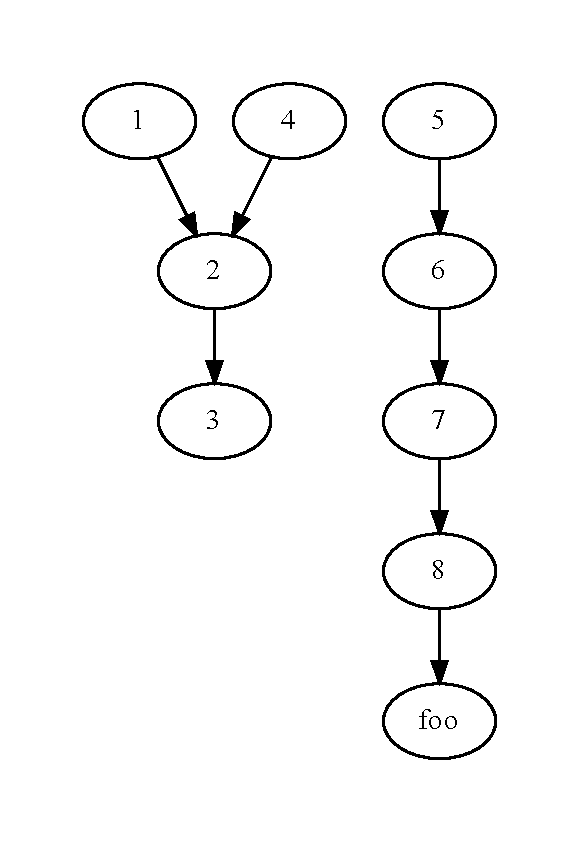
\includegraphics[scale=0.5]{cfg.pdf}
        \end{center}
        \caption{Initial CFG}
\label{fig:cfg0}
\end{figure}
Hypothetically circumscribing over the $\pred{successor}{\cdot, \cdot}$ predicate representing known transitions gives us a ``complete'' control flow graph to pass to a value analysis.
This circumscription assumed that $\forall{X}. \neg \pred{successor}{3, \var{X}}$.
However, the value analysis will quickly determine that \texttt{eax} may hold 4, and so finds $\pred{successor}{3, 4}$.
At this point, the informal version of this analysis reasons that since $\neg \pred{successor}{3, 4}$ contradicts itself, the next step is to assume $\pred{successor}{3, 4}$.\footnote{\
        It is actually possible to avoid reasoning from contradiction here: since VSA\cite{vsa} will only widen its value upper bound in response to new edges, and new edges are being discovered via these upper bounds, at a minimum those edges found in the current graph will be found in the true graph.
        However, VSA is still nonmonotonic, since the upper bounds it produces are invalidated (since they could become wider).
        Without modeling a property only present in composition, contradiction-based reasoning is unavoidable.
}

%   * Why is this call-CC?
One way to express such an ability would be to tie it to the law of excluded middle: $A \vee \neg A$.
However, an equivalent property $((A \imp \bot) \imp A) \imp A$ better captures the action of the evaluation procedure conceptually.
First, the evaluator guesses that $A$ cannot happen during the circumscription, i.e. $(A \imp \bot)$.
From that, it derives $A$.
As a result, outside the circumscribed world, we want $A$ to be visible as a fact.

% Bidirectional Proof Search
\section{Bidirectional Proof Search}
\label{sec:bidisearch}
In the background, I reviewed forwards (\S~\ref{sec:fchain}) and backwards (\S~\ref{sec:bchain}) chaining analyses.
Which to use is generally selected situationally, but I argue that for our use case, both are needed.
% * Forwards chaining = datalog
\subsection{Forwards Chaining}
Forwards chaining corresponds to the simpler ``do this when possible'' style of of organization that program analysis authors are likely more familiar with.
%   * Want this to represent things which
%     * Almost always need to be done
It is good for representing things that will nearly always need to be done,
%     * Can be done efficiently
can be done efficiently,
%     * Have a reasonably bounded extent
and whose extent is reasonably bounded.
If the analysis does not usually need to be done, it will fire when it does not need to.
If it cannot be done efficiently, it will burn resources that may be needed elsewhere.
If its extent is not reasonably bounded, the analysis will pollute the database with a large morass of facts.

%   * Examples
There are several good examples of analyses which fit the forward chaining mold well.
%     * Parse
Parsing the binary container format will need to be done before nearly every other kind of analysis, is quite fast, and will produce facts bounded linearly in the size of the input binary.
%     * Lifting
Lifting of an address identified as executable will nearly always be needed to make any further queries about it, is a constant time operation per address, and produces a bounded data value.

%   * Good for preprocessing/directed auto-analysis
Overall, forwards chaining gives a good representation of what is normally viewed as preprocessing or auto-analysis.

% * Backwards chaining = prolog
\subsection{Backwards Chaining}
Backwards chaining corresponds to the ``do this when needed'' strategy of execution analogous to what occurs in user facing analysis tools or program property checker.
%   * Want this to represent things which
Backwards chaining is more appropriate for representing analyses which
%     * Rarely need to be done
are rarely needed,
%     * Are potentially expensive
are potentially expensive to run,
%     * Have an enormous or infinite extent
or have a large (or infinite) extent.

%   * Examples
While I expect most basic functionality to work well as forward-chaining analyses, some standard techniques simply do not fit well with it.
%     * Fuzz
Fuzzing is possibly one of the clearest cases.
A fuzzing run generates a vast amount of data, and can potentially generate an arbitrary amount by triggering with new random values.
These runs are also generally expensive.
%     * Solve this function for stack overflow with symex + smt
Another example of an analysis that fits better with backwards chaining is property checking via symbolic execution and SMT solving.
While the extent is small, it is potentially slow and has a wide variety of potential entry points/properties, very few of which are actually interesting.
% * Execution strategy
\subsection{Execution Strategy}
While my execution strategy is largely informed by my implementation strategy, it still reflects similar semantics to what is seen in the inspiration languages.
%   * Queries / rule firing acts as a transaction, multiple may be in flight
First, rule firings are treated as transactions, with conflicts being negotiated by the database.
This allows for a good deal of parallelism because with the exception of circumscription, no conflicting writes should occur to the database.
The one apparent downside of this is that analyses may potentially need to be rolled back (especially if they take longer to finish) if the database had a conflicting update via a circumscription.
However, had the same operations been performed in order, the run would still have been invalidated eventually.
In parallel, using transactions, Holmes will
\begin{itemize}
%   * Try to fire any legal forwards chaing rules until quiescence
\item Run any forwards chaining rules which have new body matches. 
%   * If a query is received
\item If a query is recieved,
        \begin{enumerate}
%     * Output known matches
                \item Output known matches
                \item Add a goal root to the database for the given goal if not already present.
                \item Upon a request for more, give any new results present to the client
                \item Upon termination, decrement the goal root refcount or remove it if this is the only request.
        \end{enumerate}
\item Perform a tabling backwards search\footnote{\
                Strategy is to be decided, but may be anything from rule order to previous execution time, to a learning system.
        } for any root goals whose search has not been completed.
\end{itemize}

\section{Implementation Strategy}
\label{sec:impl}
As I've begun the implementation of this system, I have already made several design decisions.

% * Lang = rust
%   * Safe
%   * Efficiently handles large data
%   * Threading story
For implementation of the logic engine itself, I have decided to use Rust\cite{rust}.
Rust is a safe, multithreaded language which provides C/C++ style direct control of allocation, copies, and other such processes.
This means that while I will not suffer as much overhead as more traditional safe languages, I will not be plagued by the issues I had with an initial C++ prototype.\footnote{\
        Combining C++ closures for asynchronous callbacks with multithreading brings up a number of surprising edge cases, none of which are checked for by the compiler.
        This was consuming too much development time, and I forecasted it would only get worse.
}

% * Database engine = postgres
To hold the data, I've selected Postgres.
%   * Transactions (multiple rules in flight)
%   * Joins (avoid writing a custom query compiler for match terms, just compile to joins)
Like most modern SQL systems, Postgres supports transactions and joins.
Transactions are important to allowing multiple rules in flight, as they provide clean synchronization.
Joins allow me to compile the match clauses of rules into SQL queries, substantially speeding up search in larger databases.\footnote{\
        An earlier naive in-memory prototype was actually much slower despite the faster access speed.
I made the decision to use a database layer when I realized the indexing code I was about to begin writing was roughly equivalent to the code in a standard SQL database.
}
%   * Efficient jsonb support for custom user data structures
Finally, Postgres is unique in providing efficiciently indexable, binary stored \texttt{JSON} objects through its \texttt{jsonb} extension.
While this will not be required initially, it will make allowing user defined datatypes, especially ASTs and similar structures, much easier later.

% * RPC system = Cap'n'proto
To bind analyses to the logic engine to allow their functions to be called, I either need to link them in, load shared libraries, or use an RPC system.
I ruled out linking in to allow for interpreted languages and avoid recompilation.
Plugins (shared library building) were ruled out because they are tricky for potential developers to build, and would again rule out interpreted languages.
As a result, \sysname\ requires an RPC system.
To fill this gap, I selected Cap'n Proto\cite{capnproto}, a system from a creator of Google's Protobuf\cite{protobuf}.
The primary reasons for selecting Cap'n'proto were multilanguage support, capability support, efficiency, and embeddability of dynamic structures.
Supporting many languages will ease the writing of analyses for \sysname.
Capability support both allows analyses to easily follow a ``registration'' pattern (sending an object to the server constructed with the relevant callbacks), and allows for lazy reading of large values such as traces or process image dumps.
Efficiency of the encoding is important to allow for the transfer of larger objects involved in binary analysis, such as traces\footnote{\
Traces are regularly many gigabytes in size.
}
The ability to embed dynamic structured binary data through reflection will make it easier to support analysis-defined types later on in the effort.

% * See impl in progress at my github
You can view the implementation in progress on GitHub.\footnote{\url{http://github.com/maurer/holmes}}
